\documentclass{beamer}
% \usetheme{Warsaw}
% \usetheme{Dresden}
% \usetheme{Berlin}
\usetheme{Berkeley}
% \usetheme{AnnArbor}
% \usecolortheme{crane}
\usecolortheme{spruce}
% \usecolortheme{orchid}
% \usecolortheme{seagull}
% \usecolortheme{seahorse}
% \usecolortheme{structure}
% \usecolortheme{whale}
% \usecolortheme{wolverine}
% \usecolortheme{dolphin}
% \usecolortheme{dove}
% \usecolortheme{fly}
% \usecolortheme{beaver}
% \usecolortheme{lily}
% \usecolortheme{sidebartab}
% \usecolortheme{rose}

\newcommand{\R}{\mathbb{R}}
\newcommand{\C}{\mathbb{C}}
\newcommand{\HM}{\mathbb{H}}
\newcommand{\N}{\mathbb{N}}
\newcommand{\Z}{\mathbb{Z}}
\newcommand{\Q}{\mathbb{Q}}
\newcommand{\E}{\mathbb{E}}
\newcommand{\G}{\mathcal{G}}
\newcommand{\V}{\mathcal{V}}

\newcommand{\bv}[1]{\boldsymbol{#1}}
\newcommand{\gs}[1]{\langle #1 \rangle}
\newcommand{\g}[2]{\langle #1 \rangle_{#2}}

% \setbeamertemplate{theorems}[numbered]
% \setbeamertemplate{definitions}[numbered]

\addtobeamertemplate{navigation symbols}{}{%
    \usebeamerfont{footline}%
    \usebeamercolor[fg]{footline}%
    \hspace{1em}%
    \insertframenumber/\inserttotalframenumber
}

\usepackage{caption}
\newcommand\FourQuad[4]{%
    \begin{minipage}[b][.43\textheight][t]{.47\textwidth}#1\end{minipage}\hfill%
    \begin{minipage}[b][.43\textheight][t]{.47\textwidth}#2\end{minipage}\\[0.5em]
    \begin{minipage}[b][.43\textheight][t]{.47\textwidth}#3\end{minipage}\hfill
    \begin{minipage}[b][.43\textheight][t]{.47\textwidth}#4\end{minipage}%
}

\usepackage[utf8]{inputenc}
\usepackage{tikz}
\usetikzlibrary{calc, patterns, angles, quotes}

\title{Geometric Algebras}
\subtitle{BSc. Seminar}
\author{Marcelo Guimarães Neto}
\institute{University of Helsinki}
\date{\today}
% \logo{
% 
\includegraphics[width=1.65cm]{hy.png}
% } % looks terrible

\begin{document}

\begin{frame}
\titlepage
\end{frame}

\begin{frame}
\frametitle{Outline}
\tableofcontents
\end{frame}

\section{Background}
% \subsection{Historical Developments}

% \begin{frame}
% \frametitle{Historical Background (early 1800s)}
% \begin{columns}[T]
%     \pause
%     \column{0.5\textwidth}
%     \textbf{Hamilton}\\
%     Extends the complex numbers into quaternions, aiming at a formal vector algebra for $\mathbb{R}^3$, effectively representing (rotations in) 3D space:
%     \begin{align*}
%         &q = q_0 + q_1\boldsymbol{i} + q_2\boldsymbol{j} + q_3\boldsymbol{k}\\
%         &i^2 = j^2 = k^2 = ijk = -1\\
%         &ij = k, ki = j, jk = i
%     \end{align*}
%     Product of two 'vectors':
%     \[-\sum v_iu_i + \sum_{i\to j\to k}(v_iu_j - v_ju_i)\boldsymbol{k}\]
    
%     \pause
    
%     \column{0.5\textwidth}
%     \textbf{Grassmann}\\
%     First formulation of 'modern' linear algebra (vector spaces, bases, inner product and orthogonality) as well as the outer product:
%     \begin{align*}
%         &\bv{e_i} | \bv{e_j} = \delta_{ij}\\
%         &\bv{e_i}\wedge \bv{e_j} = -\bv{e_i}\wedge \bv{e_j}\\
%         &\boldsymbol{v} = \sum v_i\boldsymbol{e_i}, \boldsymbol{u} = \sum u_j\boldsymbol{e_j}
%     \end{align*}
%     The outer products of linearly independent vectors represents their linear span.
% \end{columns}
% \end{frame}

% \begin{frame}
% \frametitle{Historical Background (late 1800s)}
% \begin{columns}[T]
%     \column{0.5\textwidth}
%     \textbf{Gibbs-Heaviside}\\
%     Separates the product of quaternion 'vectors' into dot and cross products; formally replaces the imaginary units with the unit vectors.\\
%     \vspace{0.5em}
%     Development of standard vector calculus (e.g. $\nabla, \nabla \cdot, \nabla \times$), applied extensively in Electrodynamics, leading to the widespread adoption of the formalism.
    
%     \pause
    
%     \column{0.5\textwidth}
%     \textbf{Clifford}\\
%     Extends Grassmann's work into his Geometric Algebra, incorporating Hamilton's quaternions into an abstractable and generalizable algebraic system for vectors, based on the geometric product:
%     \begin{align*}
%         &uv = u | v + u \wedge v\\
%         &V = \sum \langle V\rangle_i\\
%         &\g{V}{r} = \sum v_i\bv{e_{i_1}}\wedge ... \wedge \bv{e_{i_r}}
%     \end{align*}
% \end{columns}
% \end{frame}

\setlength{\belowdisplayskip}{0pt}
\setlength{\abovedisplayskip}{0pt}
% \subsection{Abstract Algebra}
\begin{frame}
\frametitle{Algebras, Substructures, Homomorphisms}
\onslide<1->{
    \begin{definition}[Algebra]
        A real algebra $A$ is a real vector space equipped with a bilinear product; i.e.: a set closed under two operations ($+, \cdot: A\times A \to A$) and an action ($*: \R \times A \to A$), with the properties:
        \[\begin{alignedat}{3}
            &+ &&: \ &&\text{associative, invertible, commutative}\\
            &\cdot &&: \ &&\text{bilinear}: (a*x + y)\cdot (b*z + t) = \\
            & && &&= ab*xz + a*xt + b*yz + yt  \\
            &* &&: \ &&\text{associative, distributive}
        \end{alignedat}\]
    \end{definition}
}

\onslide<2->{
    \begin{block}{Examples}
        $\R, \ \C, \ \HM, \ (\R^3, +, \times, *), \ \R[X]$
    \end{block}
}
\end{frame}

\begin{frame}
\frametitle{Substructures and Homomorphisms}
\begin{definition}[Subalgebra]
    A subalgebra is a subset of an algebra which is closed under the operations and the action.
\end{definition}

\begin{definition}[Homomorphisms]
    A homomorphism is a structure-preserving mapping between two algebraic strucutures, i.e. $\phi: A \to B$ s. that:
    \[\varphi(a*xz+y) = a*\varphi(x)\varphi(z) + \varphi(y)\]
    If the mapping is 1-to-1, we call it an isomorphism.
\end{definition}
\begin{theorem}[Basis defines the algebra]
    A linear map $\varphi: A \to B$ is a homomorphism iff for every basis vector: $\varphi(e_ie_j) = \varphi(e_i)\varphi(e_j)$
\end{theorem}
\end{frame}
\setlength{\belowdisplayskip}{\baselineskip}
\setlength{\abovedisplayskip}{\baselineskip}

\section{Definitions and Properties}
% \subsection{Axioms}
\begin{frame}
% \setbeamercovered{transparent}
\frametitle{Axioms of Geometric Algebra}
A \textit{Real (Finite) Geometric Algebra} is a set $\G(\V)$ satisfying:
\onslide<1->{
    \begin{block}{Axiom 1}
        $\G(\V)$ is a unitary associative algebra.
    \end{block}
}
\onslide<2->{
    \begin{block}{Axiom 2}
        $\G(\V)$ contains $\R$ and the real (finite) vector space $\V$ as subspaces; these generate the entire algebra.
    \end{block}
}
\onslide<3->{
    \begin{block}{Axiom 3}
        The square of any vector is a real number.
    \end{block}
}
\setlength{\belowdisplayskip}{0pt}
\setlength{\abovedisplayskip}{0pt}
\onslide<4->{
    \begin{block}{Axiom 4}
        The symmetrized product on $\V$ is nondegenerate, i.e.:
        \[vu + uv = 0 \ \forall u \in \V \iff v = 0\]
    \end{block}
}
\setlength{\belowdisplayskip}{\baselineskip}
\setlength{\abovedisplayskip}{\baselineskip}
% \setbeamercovered{invisible}
\end{frame}

% \subsection{Elements}
% \begin{frame}
% \frametitle{Elements of $\G(\V)$}
% \onslide<1->{
%     \begin{block}{Identities}
%         As a unitary algebra, $\G(\V)$ has unique additive and multiplicative identities: $0, 1 \in \R \subset \G(\V)$
%     \end{block}
% }
% \onslide<2->{
%     \begin{block}{Scalars}
%         We refer to reals $a \in \R \subset \G(\V)$ as scalars, or $\textit{grade-0}$ vectors.
%     \end{block}
% }
% \onslide<3->{
%     \begin{block}{1-vectors}
%         Elements $v \in \V \subset \G(\V)$ are called 1-vectors, or simply vectors.
%     \end{block}
% }
% \end{frame}

% \begin{frame}
% \frametitle{Elements of $\G(\V)$}
% \onslide<1->{
%     \begin{block}{k-blades}
%         Products $\bv{e_1}\bv{e_2}...\bv{e_k}$ of k anticommuting vectors; we say that a k-blade has grade k.
%     \end{block}
% }
% \onslide<2->{
%     \begin{block}{k-versors}
%         Arbitrary products $\bv{v_1}\bv{v_2}...\bv{v_k}$ of k vectors.
%     \end{block}
% }
% \onslide<3->{
%     \begin{block}{Multivectors}
%         Finite sums of versors. By axiom (2), every element $V \in \G(\V)$ is a multivector. We say $A$ is a \textbf{homogeneous} (or simple) multivector iff it is a sum of k-blades for a given $k \in \N$; otherwise we say $A$ is of mixed grade.
%     \end{block}
% }
% \end{frame}

% \subsection{Products}
% \begin{frame}
% \frametitle{Vector Products: Inner, Outer and Geometric}
% \onslide<1->{
%     \begin{definition}[Inner Product]
%         The symmetrized product $u | v \equiv \frac{1}{2}(uv + vu)$ between two vectors is a (pseudo) inner product on $\V$.
%     \end{definition}
% }
% % \only<2>{
% %     \begin{proof}
% %     Axioms (1) and (4) imply it is bilinear, nondegenerate and by definition symmetric; we show it maps into $\R$:
% %         \begin{align*}
% %             &(v+u)^2 = v^2 + u^2 + vu + uv \Leftrightarrow \\
% %             &vu + uv = (v+u)^2 - v^2 - u^2 \in \R \mathrm{\ (A3)}
% %         \end{align*}
% %     \end{proof}
% % }
% \onslide<2->{
%     \begin{definition}[Outer Product]
%         We define the outer product of two vectors as the anti-symmetrized product $u \wedge v \equiv \frac{1}{2}(uv - vu)$.
%     \end{definition}
% }
% \onslide<4->{
%     \begin{block}{Remark (Geometric Product)}
%         The geometric product between vectors can thus be written:
%         \[uv = u | v + u \wedge v\]
%     \end{block}
% }
% \end{frame}

% \begin{frame}
% \frametitle{Homogeneous Products}
% \setlength{\belowdisplayskip}{0.5\baselineskip}
% \setlength{\abovedisplayskip}{0.5\baselineskip}
% \onslide<1->{
%     Between homogeneous multivectors, the product can be shown to decompose as:
%     \[A_rB_s = \g{A_rB_s}{|r-s|} + \g{A_rB_s}{|r-s|+2} + ... \g{A_rB_s}{r+s-2} + \g{A_rB_s}{r+s}\]
% }
% \onslide<2->{
%     \begin{block}{Definitions}
%         Generalized Inner Product:
%         \[A_r | B_s \equiv \g{A_rB_s}{|s-r|}\]
%         %represents the orthogonal complement of the smaller space in the larger space (left\right)
%         Generalized Outer Product:
%         \[A_r \wedge B_s \equiv \g{A_rB_s}{r+s} = a_1\wedge ...\wedge a_r\wedge b_1\wedge ... \wedge b_s\]
%         %represents the direct sum of the spaces
%         Scalar Product:
%         \[A_r * B_s \equiv \gs{A_rB_s}\]
%     \end{block}
% }
% \setlength{\belowdisplayskip}{\baselineskip}
% \setlength{\abovedisplayskip}{\baselineskip}
% \end{frame}
\section{Euclidean 3D space}
\setlength{\belowdisplayskip}{0pt}
\setlength{\abovedisplayskip}{0pt}
\begin{frame}
\frametitle{The Standard Geometric Algebra of $\R^3$}
We define the geometric product of two vectors in $\G(\R^3)$
\[ uv = u \cdot v + u\wedge v\]
For the cartesian basis:
\[
    e_ie_j = \begin{cases}
        1 &\text{if\ } i=j\\
        e_i\wedge e_j &\text{if\ } i \neq j
    \end{cases}
\]
Elements $e_i\wedge e_j$ can be thought of as representing the rectangle spanned by the two vectors.
\begin{theorem}[Grade-Dimension]
    The maximum grade of an element of $\G(\R^3)$ is 3; moreover $\G(\R^3)$ is itself a vector space of dimension 8 with basis $\{1, e_1, e_2, e_3, e_1e_2, e_1e_3, e_2e_3, I\equiv e_1e_2e_3\}$.
\end{theorem}
\end{frame}
\setlength{\belowdisplayskip}{\baselineskip}
\setlength{\abovedisplayskip}{\baselineskip}

% \begin{frame}{Pseudoscalars, Duality and Invertibility}
%     \begin{definition}[Pseudoscalar]
% \setlength{\belowdisplayskip}{0.5\baselineskip}
% \setlength{\abovedisplayskip}{0.5\baselineskip}
%     The 3-blade is unique up to scalar multiplication; we call it 'pseudoscalar' and denote it $I$ as it has the following property: \[I^2=e_1e_2e_3e_1e_2e_3=-e_1e_2e_3e_3e_2e_1=-1\]
%     The unit bivectors are pseudoscalars of their respective subspaces: $(e_ie_j)^2 = -e_ie_je_je_i = -1$
% \setlength{\belowdisplayskip}{\baselineskip}
% \setlength{\abovedisplayskip}{\baselineskip}    
%     \end{definition}
    
%     \begin{definition}[Dual]
%     The dual of a multivector: $V^* \equiv IV$
%     \end{definition}
    
%     \begin{block}{Remark (Invertibility)}
%         All vectors in $\G(\R^3)$ are invertible: $v^{-1} \equiv \frac{v}{v^2}$
%     \end{block}
    
% \end{frame}

\begin{frame}
\frametitle{Gibbs' Cross Product}
    \begin{definition}[Cross Product]
        We define the cross product between two vectors:
        \[u \times v \equiv -Iu\wedge v\]
    \end{definition}
    \begin{block}{Remark}
        This is indeed the cross product we are all familiar with, as:
        \begin{align*}
            &e_1\times e_2 = -Ie_1e_2 = e_3 \\
            &e_1\times e_3 = -Ie_1e_3 = -e_2 \\
            &e_2\times e_3 = -Ie_2e_3 = e_1
        \end{align*}
    \end{block}
\end{frame}

\begin{frame}
\frametitle{Projections, Reflections and Rotations}
\begin{block}{Reflection by an axis}
    Let $v$ be a vector which we wish to reflect through the axis represented by the vector $n$, then:
    \begin{align*}
        &v = (v|n)n^{-1} + (v\wedge n)n^{-1} \equiv P_n(v) + R_n(v)\\
        &v' \equiv -P_n(v) + R_n(v) = -nvn^{-1}
    \end{align*}
\end{block}
\begin{block}{Rotation on a plane}
    Rotation of a vector $v$ through the plane represented by $B$ is given by: $v' = RvR^{-1}$, where $R = exp(-B\theta/2)$
\end{block}
\end{frame}

\begin{frame}{Hamilton's method for rotations}
    \begin{columns}
        \column{0.5\textwidth}
            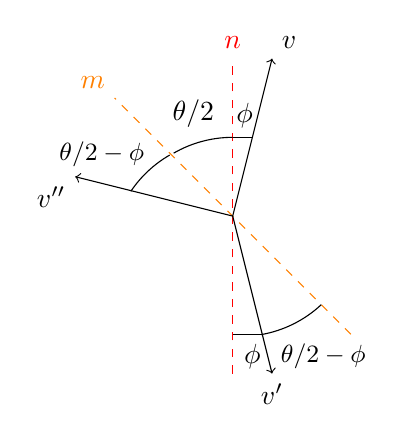
\begin{tikzpicture}[xscale=.5,yscale=.5]
                % \draw[help lines] (0,0) grid (8,10);
                \draw [dashed, red] (5,1) -- (5,9);
                \node [above, red] at (5, 9) {$n$};
                \draw [dashed, orange] (8,2) -- (2,8);
                \node [above left, orange] at (2, 8) {$m$};
                \draw (5, 7) arc [radius=3, start angle=90, end angle=120];
                \node [above] at (4, 7) {$\theta/2$};
                \pause
                \draw [->] (5,5) -- (6,9);
                \node [above right] at (6, 9) {$v$};
                \draw (5.5, 7) -- (5, 7);
                \node [above] at (5.3, 7) {$\phi$};
                \pause
                \draw [->] (5,5) -- (6, 1);
                \node [below] at (6, 1) {$v'$};
                \draw (5.75, 2) -- (5, 2);
                \node [below] at (5.5, 2) {$\phi$};
                \draw (7.25, 2.75) arc [radius=3, start angle=313, end angle=280];
                \node [below] at (7.3, 2) {\small $\theta/2 - \phi$};
                \pause
                \draw [->] (5,5) -- (1, 6);
                \node [below left] at (1, 6) {$v''$};
                \draw (3.4, 6.55) arc [radius=3, start angle=120, end angle=146];
                \node [above left] at (3, 6) {\small $\theta/2-\phi$};
            \end{tikzpicture}
        
        \onslide<5->{
            \column{0.5\textwidth}
            The rotated vector is thus:
                \begin{align*}
                    v'' &= -m(-nvn^{-1})m^{-1} \\
                    &= (mn)v(mn)^{-1}
                \end{align*}
            We identify $mn$ as the rotor $R$; moreover, if $B$ is the unit bivector:
                \begin{align*}
                    R &= |m||n|(\cos(\theta/2) - \sin(\theta/2)B) \\
                    &\equiv |R|\exp(-B\theta/2)
                \end{align*}
            We say $B$ generates rotations in the plane and call it \textbf{spinor}.
        }
    \end{columns}
\end{frame}

% \begin{frame}
% \frametitle{Spinor subalgebra: $\G_2(\R^3) \simeq \C$}
% \begin{theorem}
%     For any choice of $(i,j) : i\neq j$, the set $\{1, e_ie_j\}$ generates a subalgebra $\G_2(\R^3)$ isomorphic to $\C$.
% \end{theorem}
% \begin{proof}
%     Consider the multiplication table of the set:
%     \begin{columns}
%         \column{0.5\textwidth}
%         \begin{center}
%             \renewcommand\arraystretch{1.3}
%             \setlength\doublerulesep{0pt}
%             \begin{tabular}{|r|||r|r|}
%             \hline
%             $\cdot$ & 1 & $e_ie_j$ \\
%             \hline\hline\hline
%             1 & 1 & $e_ie_j$ \\ 
%             \hline
%             $e_ie_j$ & $e_ie_j$ & -1\\ 
%             \hline
%             \end{tabular}
%         \end{center}
    
%     \column{0.5\textwidth}
%         It is clear that the isomorphism is given by $e_ie_j \longleftrightarrow i$.
%     \end{columns}
% \end{proof}
% \end{frame}

\begin{frame}
\frametitle{Spinor subalgebra: $\G_+(\R^3) \simeq \HM$}
\begin{theorem}
    The set of even grade elements $\{1, e_ie_j: i\neq j\}$ generates a subalgebra $\G_+(\R^3)$ isomorphic to $\HM$.
\end{theorem}
\begin{proof}
    Compare multiplication tables:
    \begin{columns}
        \column{0.5\textwidth}
        \begin{center}
            \renewcommand\arraystretch{1.3}
            \setlength\doublerulesep{0pt}
            \scalebox{0.7}{
                \begin{tabular}{|r|||r|r|r|r|}
                \hline
                $\cdot$ & 1 & $e_1e_2$ & $e_2e_3$ & $e_1e_3$ \\
                \hline\hline\hline
                1 & 1 & $e_1e_2$ & $e_2e_3$ & $e_1e_3$ \\ 
                \hline
                $e_1e_2$ & $e_1e_2$ & -1 & $e_1e_3$ & $-e_2e_3$ \\ 
                \hline
                $e_2e_3$ & $e_2e_3$ & $-e_1e_3$ & -1 & $e_1e_2$\\
                \hline
                $e_1e_3$ & $e_1e_3$ & $e_2e_3$ & $-e_1e_2$ & -1\\
                \hline
                \end{tabular}
            }
        \end{center}
    
        \column{0.5\textwidth}
        \begin{center}
            \renewcommand\arraystretch{1.3}
            \setlength\doublerulesep{0pt}
            \scalebox{0.7}{
                \begin{tabular}{|r|||r|r|r|r|}
                \hline
                $\cdot$ & 1 & $i$ & $j$ & $k$ \\
                \hline\hline\hline
                1 & 1 & $i$ & $j$ & $k$ \\ 
                \hline
                $i$ & $i$ & -1 & $k$ & $-j$ \\ 
                \hline
                $j$ & $j$ & $-k$ & -1 & $i$\\
                \hline
                $k$ & $k$ & $j$ & $-i$ & -1\\
                \hline
                \end{tabular}
            }
        \end{center}
    \end{columns}
\end{proof}
\end{frame}

% \subsection{Physics}
% \begin{frame}
% \frametitle{Relativistic Electrodynamics}
% Lorem ipsum dolor sit amet, consectetur adipisicing elit, sed do eiusmod tempor incididunt ut labore et dolore magna aliqua.
% \end{frame}

\section{Conclusion}
\begin{frame}
\frametitle{Conclusion}
% \begin{columns}[T]
% \column{0.5\textwidth}
    \textbf{Advantages}
    \begin{enumerate}
        \item Generalizes Gibbs' algebra for $\R^3$ to any dimension
        \pause
        \item Contains $\C$ and $\HM$ as subalgebras, so it handles rotations and orientations elegantly and efficiently
        \pause
        \item Unifies objects and transformations into a single algebra
        \pause
        \item Geometric intuition
        \pause
        \item Simplifies algebraic manipulations of vectors
    \end{enumerate}
% \column{0.5\textwidth}
%     \textbf{Disadvantages}
%     \begin{enumerate}
%         \item Requires working with a large number of different objects
%         \pause
%         \item Depends on a quadratic form, so it is not applicable in more abstract topological settings
%         \pause
%         \item Requires embedding manifolds into a higher dimensional Euclidean space
%     \end{enumerate}
% \end{columns}
\end{frame}

\begin{frame}
\frametitle{References and Additional material}
\only<1>{
\begin{block}{Historical background and Geometric intuition}
    \begin{enumerate}
        \item Chappell, J. \& Iqbal, A. \& Hartnett, J. \& Abbott, D. 2016. \textit{The Vector Algebra War: A Historical Perspective}. IEEE Access. 4. 1997-2004. 10.1109/ACCESS.2016.2538262. 
        \item sudgylacmoe (2020) \textit{A Swift Introduction to Geometric Algebra}. 17 August. Available at: \url{https://www.youtube.com/watch?v=60z_hpEAtD8&t=2076s} (Accessed: 20 February 2022).
        \item Marc ten Bosch (2020) \textit{Let's remove Quaternions from every 3D Engine: Intro to Rotors from Geometric Algebra}. 30 January. Available at: \url{https://www.youtube.com/watch?v=Idlv83CxP-8} (Accessed: 20 February 2022).
    \end{enumerate}
\end{block}
}
\only<2>{
\begin{block}{Literature}
    \begin{enumerate}
        \item Chisolm, E., 2012. \textit{Geometric Algebra}. arXiv:1205.5935
        \item Hestenes, D. and Sobczyk, G., 1984. \textit{Clifford Algebra to Geometric Calculus}. Dordrecht: Springer Netherlands.
        \item Doran, C. and Lasenby, A., 2003. \textit{Geometric algebra for physicists}. Cambridge: Cambridge University Press.
        \item Hestenes, D., 2002. \textit{New Foundations for Classical Mechanics}. 2nd ed. New York, Boston, Dordrecht, London, Moscow: Kluwer Academic Publishers.
    \end{enumerate}
\end{block}
}
\end{frame}

\begin{frame}{Questions?}
    
\end{frame}

\end{document}